\documentclass[12pt]{article}

\usepackage{graphicx}
\usepackage{listings}
\usepackage{hyperref}
\usepackage{float}
\usepackage{enumitem}

\graphicspath{ {./images/} }

\oddsidemargin 0mm
\evensidemargin 0mm
\textwidth 160mm
\textheight 200mm

\pagestyle {plain}
\pagenumbering{arabic}

\newcounter{stepnum}

\title{CS/SE 2XC3 Lab 9 Report}
\author{
  Glotov, Oleg\\ L03, 400174037\\
  \texttt{glotovo@mcmaster.ca}
  \and
  Willson, Emma\\ L02, 400309856\\
  \texttt{willsone@mcmaster.ca}
  }
\date{\today}

\begin{document}

\maketitle

This report includes the main observations that we found in this week's lab, along with the analysis of our results.

\newpage 
\section{Shortest Path}
In this section, we discuss algorithms for finding the shortest path in directed weighted graphs, potentially with negative edge weights. 
\subsection{Bellman-Ford Approximation}
In this implementation of the Bellman-Ford algorithm, there is an array of counters that keeps track of how many times the line \verb+dist[neighbour] = dist[node] + G.w(node, neighbour)+ is run on each node. When the count for a node surpasses the input value $k$, the algorithm stops updating the shortest distance to that node.\\
We tested our approximation of Bellman-Ford using connected graphs of size $n=100$ (where $n$ is the number of nodes) with edge weights randomly chosen between 1 and 1000.
The testing method used was consistent with earlier labs. We used \verb+create_random_connected_graph()+ to generate a random graph given a number of nodes and maximum edge weight. For each $k$ value, the algorithm was tested three times.
\subsection{List vs. Min Heap}
The most expensive functions in the implementation of Prim's algorithm are finding and updating the weight of the minimum edge. Our first implementation uses a list of edges that are sorted by weight. The algorithm re-sorts this list for every edge visited. The Python \verb+sort()+ function has a time complexity in $O(nlogn)$. Our second implementation uses a heap of nodes that are sorted by edge weight. The heap property is maintained using \verb+extract_min+ and \verb+decrease_key+, so there is no need to sort. Both of these functions are in $O(logn)$ The difference between these implementations is that the first one visits each edge, while the second visits each node. As the graph becomes more densely connected, visiting nodes (v2) becomes less efficient than visiting edges (v1). However in a sparse graph with a large number of nodes, using a min heap of nodes is faster. That's why we expect v2 to perform significantly better on large, sparse graphs.
\begin{figure}[H]
\centering
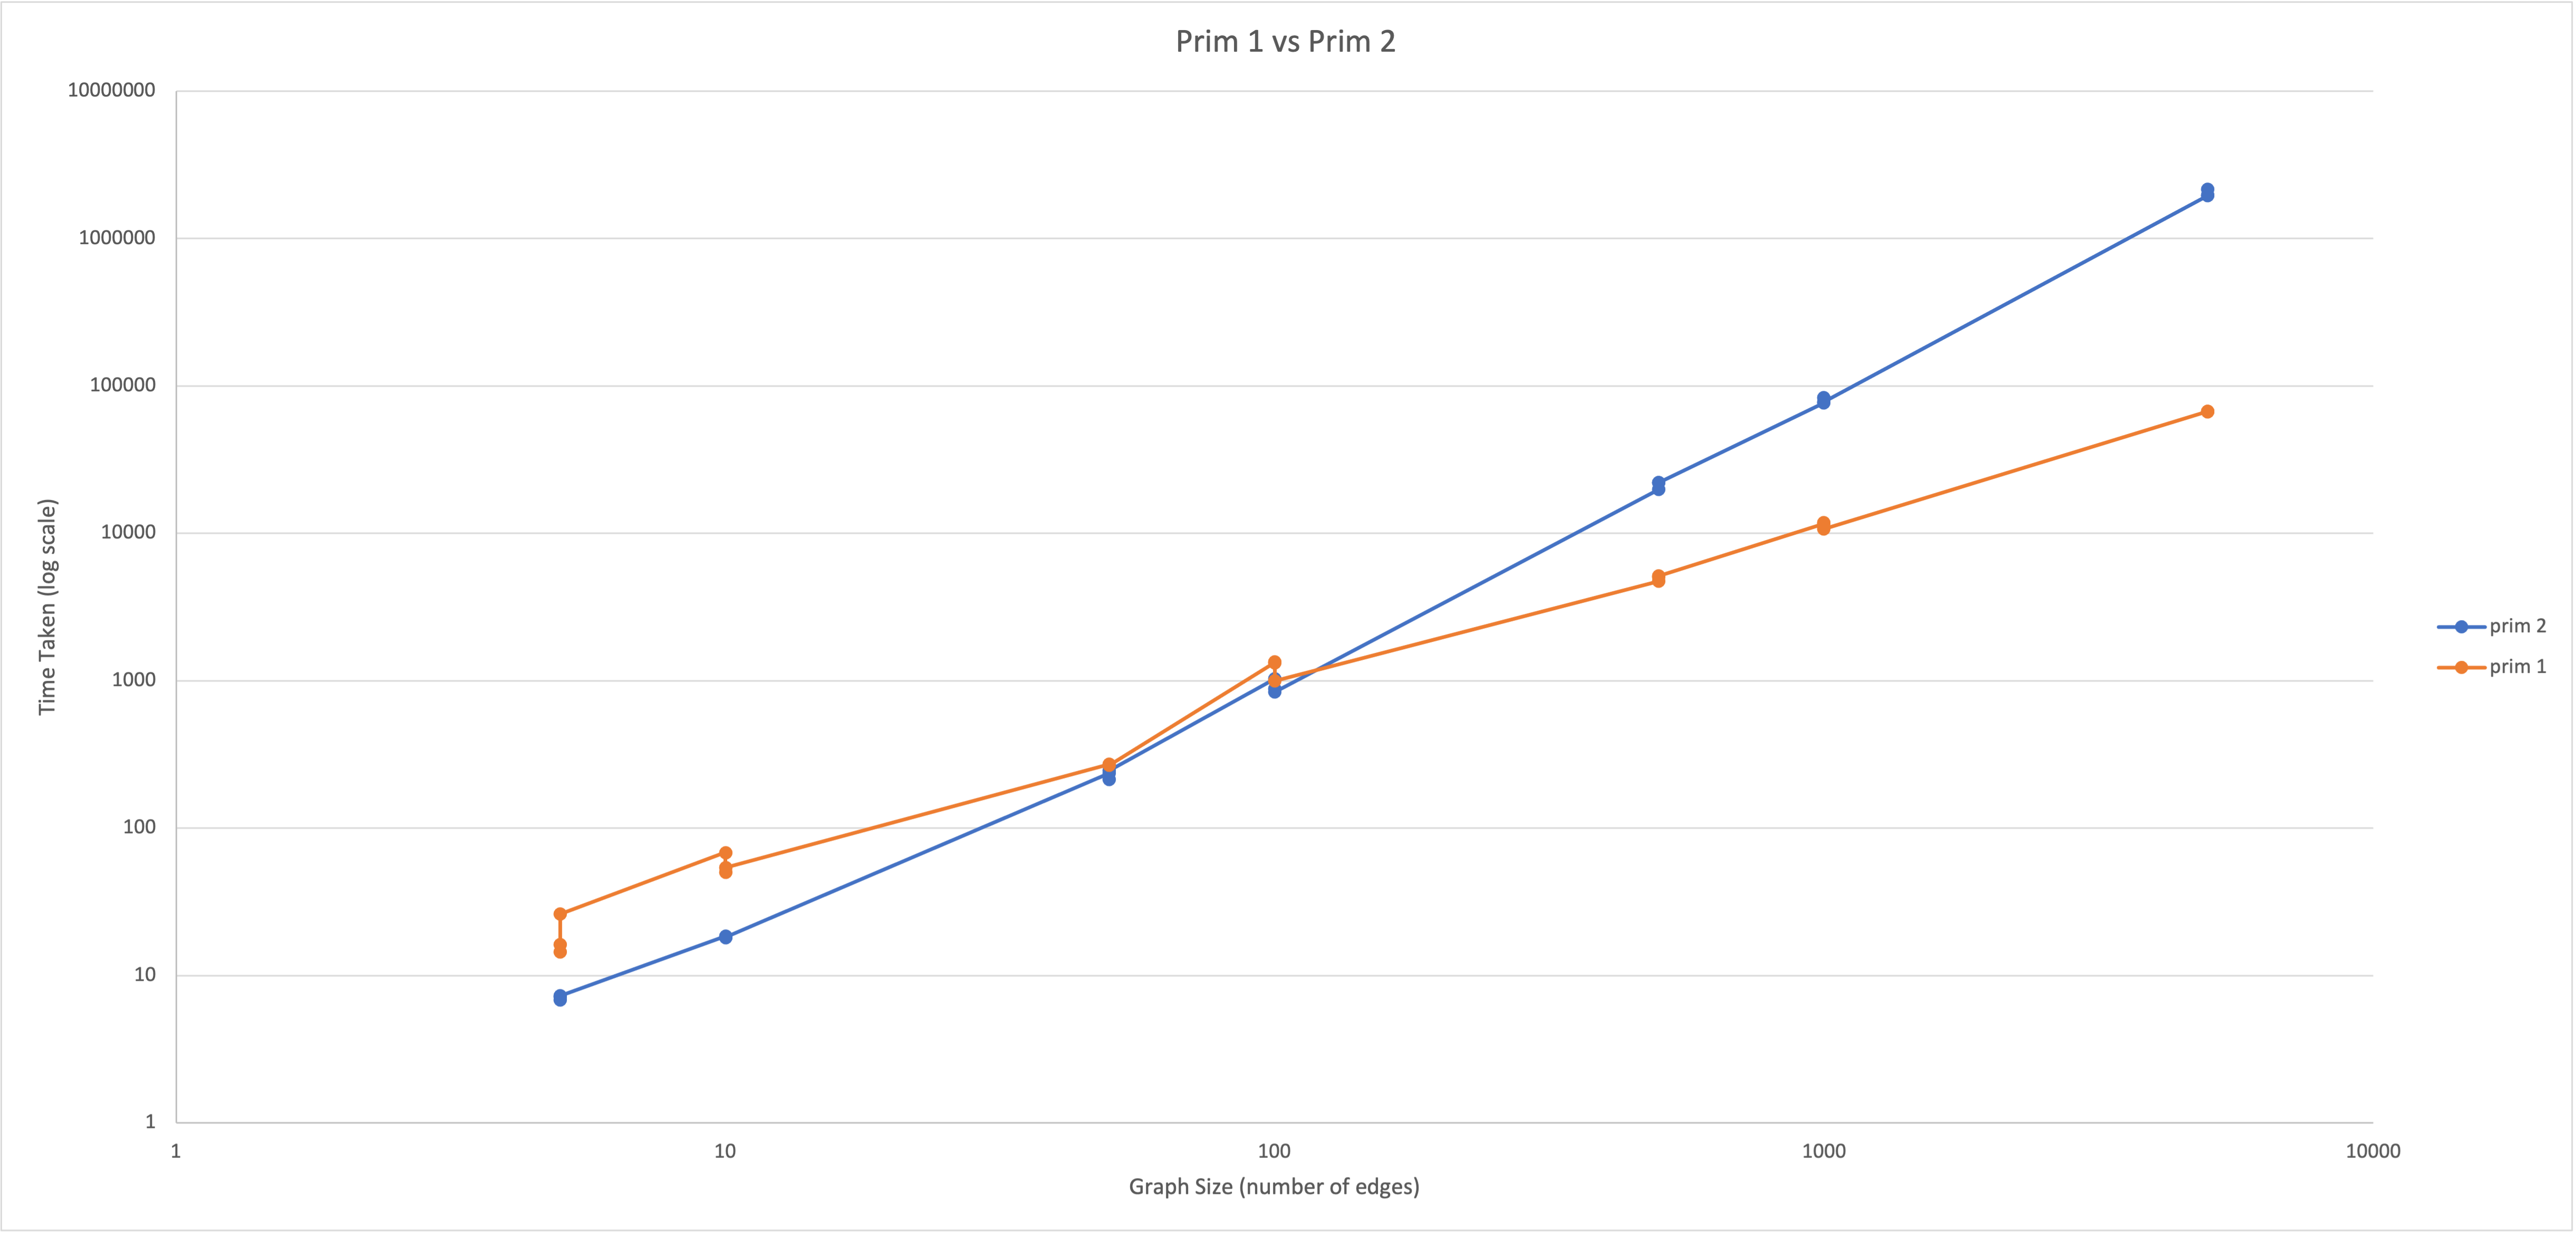
\includegraphics[width=0.7\textwidth,height=\textheight,keepaspectratio]{prim1and2.png}
\caption{time complexity of prim v1 vs. prim v2}
\label{Figure: m1}
\end{figure}
\noindent The graph above shows that the second implementation outperforms the first after graph sizes of around 100. Sorting vast arrays becomes significantly slower at larger array sizes than rearranging a Min heap which was explained earlier. This effect is clearly seen in the graph. 



\end{document}

